\documentclass[runningheads]{llncs}
%
\usepackage{graphicx}
% Used for displaying a sample figure. If possible, figure files should
% be included in EPS format.
%
\usepackage{amsmath}
%
% If you use the hyperref package, please uncomment the following line
% to display URLs in blue roman font according to Springer's eBook style:
\usepackage{hyperref,xcolor}
\renewcommand\UrlFont{\color{blue}\rmfamily}

\begin{document}
%
\title{Impact of switching bug trackers: a case study}
%
%\titlerunning{}
% If the paper title is too long for the running head, you can set
% an abbreviated paper title here
%
\author{Th\'eo Zimmermann\inst{1,2} \and
Annal\'i Casanueva Art\'is\inst{3}\thanks{This work was partly funded by El Conacyt of the Mexican government.}}
%
\authorrunning{T. Zimmermann and A. Casanueva Art\'is}
% First names are abbreviated in the running head.
% If there are more than two authors, 'et al.' is used.
%
\institute{$\Pi R^2$, Inria, Paris, France \and
IRIF, Paris-Diderot University, Paris, France\\
\email{theo@irif.fr} \and
Paris School of Economics, Paris, France}
%
\maketitle              % typeset the header of the contribution
%
\begin{abstract}
Any significant software project requires a bug tracker. In open source development, this plays an even bigger role. The impact of the bug reporting environment on the bug tracking activity is difficult to assess. In this paper, we take advantage of the switch from Bugzilla to GitHub of the bug tracker of Coq, a medium-sized open source project, to evaluate the impact that such a change can have. 
We first report on the switch itself, in particular the migration of 4900 preexisting bug reports using the GitHub issue import API; then we analyze data from before and after the migration. We show that the switch induces 
an increase in bug reporting, particularly from principal developers themselves, and more generally an increased engagement with the bug tracking platform, with more comments by developers and also more external commentators.

%The abstract should briefly summarize the contents of the paper in 15--250 words.

\keywords{bug tracker \and switch \and migration  \and bug report \and issue \and GitHub \and Bugzilla \and open source.}
\end{abstract}
%
%
%
\section{Introduction}

Bug reporting is an essential part of software development. However, it involves
a non-negligible human component, particularly in the context of an open source project where a larger part of bugs are reported by independent users and therefore depend a lot on the good will of individuals. Creating an environment that makes bug reporting easier and more appealing may lead to an increase of bug reporting (from both developers and independent users) which should ultimately benefit  software development \cite{Bettenburg2008} (provided that developers are equipped to handle the incoming reports \cite{Anvika,Kanwal2012}). However, the impact of such change has rarely been studied. Indeed, comparing the number of bug reports in different environments is generally not compelling because it is likely to depend  not just on the reporting environment but also on each particular software and its development dynamics. To do a valid comparison one would ideally need to compare two bug reporting environments for the same software, in the same period. But, or course, we can't observe this ideal. A context approaching this ideal scenario would be to compare the number of bug reports of a particular software before and after the switch to a new environment. Yet, substantial changes in the environment of bug reporting (e.g. changes of bug tracker platform) are rare because once a bug system is in place, any change comes with a significant cost. 

We use the switch, from Bugzilla to GitHub, of the bug tracker system of the Coq proof assistant, a medium-sized open source software, to analyze the  effects of a change in the bug reporting environment on the number of bugs, reporters, bug comments and commentators. We describe the switch event and the associated migration process for preexisting bugs. Thanks to the way this migration was conducted, getting data on bug reporting from before and after the switch is easily done using the GitHub GraphQL API. Using a Regression in Discontinuity analysis we find strong evidence that the switch of platform increased the number of bug reports; started an increase of bug reporters per period (i.e. in a certain period there are more distinct reporters); increased the number of comments by developers and the number of distinct commentators per period among non-developers. Taken together our results suggest that switching from Bugzilla to GitHub increased the number of bug reports and bug reporters (probably by making the bug reporting process easier) but also increased the openness of software development and aroused discussion around bugs (notably between developers and non-developers).

\section{Context}

\subsection{Coq and GitHub}
Coq is a (free and open source) proof assistant, that is a software to write and automatically verify mathematical proofs (and programs). It originated as a research project in 1984 and the development team is still composed, for the most part, of researchers. It gained in popularity along the years, and is now at the center of many verification projects (some very large academic projects, and some industrial projects). Its initial developers were awarded  the ACM SIGPLAN Programming Languages Software 2013 Award and the ACM Software System 2013 award.

The development is currently centered around the GitHub platform. The current repository of Coq the current repository counts more than 25000 commits. Some of these commits date back from 1999, when the code received major architectural changes. The GitHub repository was initially created as a mirror of the official repository (which itself was migrated from SVN to git in 2013) and really started attracting the interest of the development team as a way to open up the development to external contributions, especially starting with the first Coq coding sprint in 2015 (later renamed into the Coq Implementors Workshop and held every year in France). From then on, core developers started using pull requests for their own changes more and more often, and it became the norm around the beginning of 2017 when systematic continuous integration tests were introduced on every pull requests. In the last two years, more than 2,200 pull requests have been opened.

\subsection{The Coq bug tracker}

From 2007 to 2017, the Coq bug tracker platform was a self-hosted Bugzilla instance (before this, from 2001 to 2007 it was using JitterBug, a now discontinued bug tracking system, and before 2001 a simple mailing list). In 2017, developers had become quite accustomed to the look and feel of discussion threads on GitHub pull requests, which offered a much nicer experience than the Bugzilla bug tracker. Younger developers (in particular, one of the author of this article, who eventually pushed for the switch and conducted the migration) were frustrated by what they perceived as an older and heavier platform. The rest of the developers were convinced to migrate towards a non-self-hosted solution in August 2017, when the whole Coq website was shut down for more than a week  because an IT team was frightened by a scam bug report.\footnote{\url{https://sympa.inria.fr/sympa/arc/coq-club/2017-08/msg00040.html}}

The expected advantages of the GitHub issue tracker over Bugzilla were:
\begin{itemize}
\item Better formatting, ability to edit comments, and more generally a more pleasant tool to use. We felt that Bugzilla was unpleasant enough to discourage developers to use it to its full potential.
\item Browsing between code, pull requests and bug reports is easier when everything is in the same place. Furthermore, it means a common notification, mention, and assignment system.
\item Better indexing by search engines.
\item Shared management of permissions, milestones, categories (labels), etc.
\item Easier to get started for newcomers (especially as many may already know GitHub and already have a GitHub account).
\end{itemize}

The possible drawbacks were mostly that GitHub provides a less-advanced system with very few customization options. In particular:
\begin{itemize}
\item The permission system is much less fine-grained. Giving triaging rights to users requires giving them ``write access'', which includes commit rights on non-protected branches. That's why the Coq GitHub repository now only has protected branches (and accidentally-pushed topic branches are promptly deleted).
\item Creating a new bug report doesn't require filling a form, but typing a message. Fortunately, issue templates help give some hints towards the expected structure of the report, and being able to strip this template can actually give flexibility to developers who might open new issues for concerns that do not qualify as bugs.
\item There is no import mechanism that allows to keep the number and author of preexisting reports. Fortunately, as we will see in Sec.~\ref{migration}, it was still possible to import bug reports while keeping most of the meta-information and renumbering the fewest possible bug reports. This was an important requirement for the switch.
\end{itemize}

\section{Hypotheses}

Given the advantages of the GitHub issue tracker that were listed above, we expected the switch to:
\begin{itemize}
\item increase the number of bug reports, by developers in particular;
\item increase the diversity of bug reporters;
\item improve the interaction between reporters and developers.
\end{itemize}

All of this could lead in turn to a greater openness and transparency of the development and an increased engagement of users toward it, changing (and probably improving) the dynamics of a crucial part of software development. 

\section{Migration}
\label{migration}

The only complicated part of the bug tracker switch was the migration of preexisting bug reports. We reused a tool by Andriy Berestovskyy\footnote{Tool available at \url{https://github.com/berestovskyy/bugzilla2github}.} which is designed to import Bugzilla reports (extracted as an XML dump) to GitHub using its REST API. The bugs are imported in an order designed to preserve numbers whenever possible. Bugs whose number is unavailable (e.g. because the number is already taken by a GitHub pull request) are postponed and renumbered. We implemented several improvements to make the tool better fit our needs:
\begin{itemize}
\item \textit{Allowing non-consecutive bug numbers:} Our imported set of bug reports had some holes in the numbering due to deleted bugs. We use postponed bugs to fill the holes. This improvement has now been integrated upstream.
\item \textit{Saving a table of correspondence for renumbered bugs:} This was used later to redirect the old bug URLs to the new ones.
\item \textit{Using the GitHub issue import beta API and overcoming the GitHub rate limits:} Creating a new issue or a new comment through the normal GitHub REST API will trigger notifications (for people who are watching the repository or are mentioned in the issue thread). Such actions are therefore subject to a strict rate limit which prevented using this tool for importing more than a few hundred bugs. Fortunately, GitHub provides a (beta) issue import API which, in addition to not triggering notifications, also allows importing one bug, its comments, and meta information such as closed status and assignee in a single request (thus reducing the duration to import 4900 bugs to just a few hours). Finally, using this API allows to keep the dates of imported bug reports and comments, which is very useful to this study. We didn't manage to import correct closing dates, so we won't study the impact of the bug tracker switch on the time it takes to close a bug.
\end{itemize}

This tool required a correspondence table between Bugzilla and GitHub accounts. Ours was created by manually matching 217 (out of 686) Bugzilla accounts to 175 GitHub accounts,\footnote{The correspondence table can be seen at \url{https://gist.github.com/Zimmi48/d923e52f64fe17c72852d9c148bfcdc6##file-bugzilla2github-L47-L264}.} the difference being due to the high prevalence of duplicate Bugzilla accounts. We gave priority to finding GitHub accounts for people who still had opened bug reports. The most efficient way to do the matching was by searching the name of the reporter + ``github'' on Google. We also sent e-mails to people we hadn't managed to match (and who still had opened bugs).

\paragraph{Urgency.}
Once the switch was approved by the development team on October 3-4\textsuperscript{th}, 2017, the migration had to happen as soon as possible because every new pull request before the migration added to the number of bug reports that would need to be renumbered. It was conducted\footnote{More details on the process are available in a blog post at \url{http://theoz.im/bugzilla}. } on October 18\textsuperscript{th},  the day after the 8.7.0 release (and not before to avoid disturbing the release process). Only 502 bugs (whose numbers were below 1154) had to be renumbered. This number is quite low because these bugs are dating back from the JitterBug era and during the previous switch only the bugs that were still open had been migrated.

\section{Data}

\subsection{Extraction}

All the data for this study was extracted on September 14\textsuperscript{th}, 2018 using the GitHub GraphQL API. Using this API allows to do large requests (100 nodes in a single request) with just the information we need (thus both reducing the bandwidth usage and speeding up the extraction process). We provide the extracted data as CSV files and a Jupyter notebook\footnote{Available at \url{https://github.com/Zimmi48/impact-of-switching-bug-trackers}.} with the code to request this data from GitHub, to load the CSV files, and to run the analyses.

Migrated bugs and comments had their author information stored in the text so we extract it from there. Dates of bug and comment creation have been preserved so we can obtain them transparently for bugs before and after the migration. Comments dating from the JitterBug era do not have valid author information (and closed bug reports from this era have not been migrated) so we won't consider any data from before 2008.

\subsection{Pre-processing}

\paragraph{Excluding specific reporters.}
We have one specific reporter, Jason Gross, who is alone responsible for almost a quarter of all bug reports. To avoid having the behavior of a single individual strongly impact the overall statistics, we exclude his comments, bug reports and pull requests and all the comments they received from our analysis. Similarly, we also exclude the developer who was the initiator and conductor of the bug tracker switch and migration and who is an author of this article.

\paragraph{Merging duplicate Bugzilla accounts.}
This is only relevant to the new reporter analysis which itself is only detailed in the accompanying Jupyter notebook, so refer there for more information.

\paragraph{Removal of migration artifact comments.}
The migration tool created an issue whose body contains only meta-information, and a first comment with the description, for every bug report. These comments are thus migration artifacts and we remove them from our comment analyses. They can be easily identified because they are the comments that were posted at the exact same date and time as the corresponding bug report.

\subsection{Variable definition}

Our outcome variables will be the numbers of bug reports, distinct bug reporters, new bug reporters (who had never reported a bug before), comments and distinct commentators, for a given period. We will use 15-day periods to have sufficiently many bugs by period. Indeed, in our data we have an average of 13 bug reports by 15-day period; 50\% of the periods have between 7 and 18 reports; 90\% of the periods have between 4 and 27. This also allows to have 40 observations centered around the date of the switch for our Regression in Discontinuity analyses.

We will analyze heterogeneous effects by distinguishing between developers and others (others being assimilated to ``users''). We define ``developers'' as the persons who have contributed more than 100 commits since 2008.

When studying the influence of new releases, we define the release dates by the dates of the corresponding news items on the official website (\url{https://coq.inria.fr/news}). We selected beta and major releases and excluded release candidates and patch-level releases. The first release to appear in the news section of the current official website is the 8.2beta release in June, 2008.

\section{Descriptive statistics}

The accompanying Jupyter notebook contains lots of descriptive statistics and figures, such as the distribution of bug reporting in the year, and in the day, graphs of bug reporting for individual developers, etc. We only present a subset of these figures.

\subsection{Cumulative number of bug reports and bug comments}

Fig.~\ref{cumulative_bugs_and_comments} gives a first (cumulative) view of two of our outcome variables: the number of bug reports, and the number of comments. From this figure, we can clearly notice the dominance of developers in the number of bug comments and the dominance of non-developers in the number of bug reports. We can also already notice some slope changes at the bug tracker switch date. The magnitude and significance of this changes will be assessed in the remainder of this article.

\begin{figure}
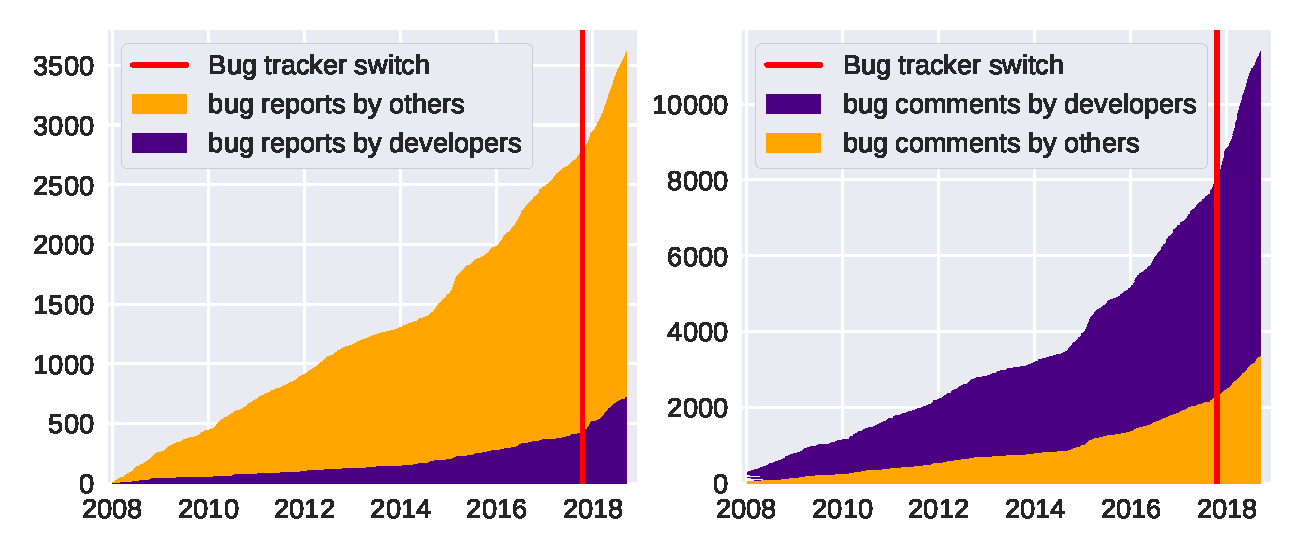
\includegraphics[width=\textwidth]{cumulative_bugs_and_comments.eps}
\caption{Cumulative number of bug reports and comments (since 2008).} \label{cumulative_bugs_and_comments}
\end{figure}

\subsection{Influence of new releases}
\label{influence_release}

\paragraph{Influence on the number of bug reports.}
We expect release dates to be correlated to peaks of activity on the bug tracker, in particular peaks of new bug reports. Indeed, users will generally test new releases, for instance by trying to port preexisting projects to the new version, which might lead them to find new bugs (either regressions or bugs related to new features). In Fig.~\ref{bug_nb_with_releases}, we can see that while release dates are generally correlated to peaks of new bug reports by non-developers, this isn't so much the case of reports by developers. We can also notice that beta releases are often correlated to higher peaks than final releases which isn't surprising given that the users who test beta versions are more likely to be ready to report bugs, and beta versions are likely to be less polished.

The highest peak is in 2015, after the first beta release of version 8.5. This was the first release in more than two years and it contained five big new features (``the result of five specific long-term projects''\footnote{Quote from \url{https://coq.inria.fr/refman/credits.html##credits-version-8-5}. The next quotes are coming from the following sections of the same chapter of the Coq reference manual.}). Stabilizing these features and their (unplanned) interactions required more than a year of testing and three beta releases. The 8.5 release was both hard on developers, who found the release cycle too long, and on users, who were impacted by many compatibility issues. Consequently, a different approach was taken for the following releases: versions 8.6, 8.7 and 8.8 were ``developed on a time-based development cycle'' and contain ``the result of refinements, stabilization of features and cleanups of the internals of the system along with a few new features''. Attention was given to regression testing by systematically testing changes by building a selection of the largest Coq projects. Therefore, it is not surprising that these frequent releases are correlated to smaller peaks of new bug reports.

\begin{figure}
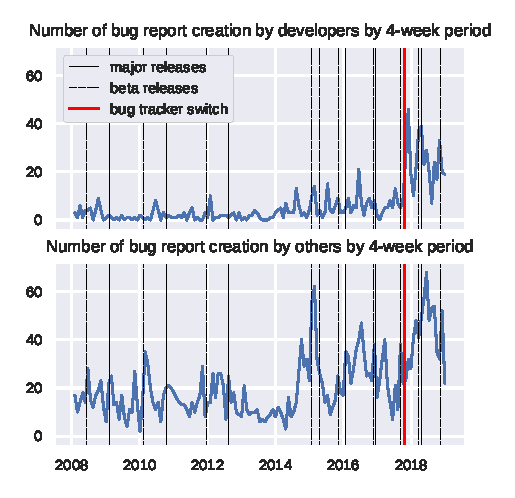
\includegraphics[width=\textwidth]{bug_nb_with_releases.eps}
\caption{Number of bug reports by 15-day period with release dates (since 2008).} \label{bug_nb_with_releases}
\end{figure}

\paragraph{Influence on the number of comments.}
In Fig.~\ref{comments_with_releases}, we can see that release dates are correlated to peaks of comments by developers (and not so much by other people). This is explained by the fact that bug reports are generally answered by developers, thus any peak in bug reporting is bound to induce a peak in bug commenting by developers.

\begin{figure}
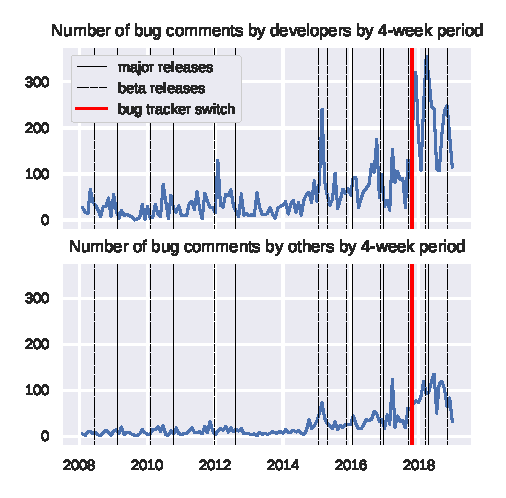
\includegraphics[width=\textwidth]{comments_with_releases.eps}
\caption{Number of bug comments by 15-day period with release dates (since 2008).} \label{comments_with_releases}
\end{figure}

\section{Methodology}

We exploit the fact that the switch to GitHub can be seen as a clear cutoff in time to use a Regression in Discontinuity approach to estimate the effects of the switch on our outcome variables, to determine if these estimated effects are statistically significant, and to interpret these effects in a causal way. 
The idea behind this analysis is that bug reporters did not choose the exact moment in which the switch would take place. In the absence of any other discontinuity, the changes in the behavior of bug reporters just before and just after the migration is likely to depend mainly on the switch even if there was a change in behavioral trends before the switch. It is important to note that estimated effects using this method will inform of the effect near the threshold. Indeed, in the same way that behavior just before and just after the threshold is not likely to be different in the absence of the switch, the behavior several periods before and several periods after is likely to be different even in the absence of the switch. See~\cite{lee2010regression} for more details on Regression on Discontinuity analysis.

We use time as running variable and we estimate the following regression:  

\begin{equation*}
\begin{aligned}
\mbox{\emph{Number of bug reports}}_p⁡ =\gamma_0 &+\gamma_1 \mbox{\emph{Relative date}}_p + \gamma_2 \mbox{\emph{After switch}}_p \\
&+ \gamma_3 \mbox{\emph{Relative date}}_p * \mbox{\emph{After switch}}_p + \epsilon_p
\end{aligned}
\end{equation*}

\noindent where $\mbox{\emph{Number of bug reports}}_p⁡$ is the total number of bugs reported during the 15-day period $p$; $\mbox{\emph{Relative date}}_p$ is the number of periods from the date of the switch (zero is the first period after the switch); $\mbox{\emph{After switch}}_p$ is a binary variable equal to one if $p$ is a period after the switch and zero otherwise; $\mbox{\emph{Relative date}}_p * \mbox{\emph{After switch}}_p$ is the interaction term and $\epsilon_p$ is the error. We estimate this regression by Ordinary Least Squares. Coefficients $\gamma_2$ and $\gamma_3$ are the estimates of interest and will tell us the jump of the number of bugs reports just after the migration and the change in trends due to the migration respectively. We estimate this regression for two different sub-samples: the developers and the non-developers. 

We replicate this analysis for all our outcome variables by changing the variable on the left hand of the equation. 

\section{Results}

\subsection{Impact on the number of bugs}

\begin{table}
\centering
\caption{Estimated impact of the switch on the number of bugs. Coefficients are highlighted if they are statistically significant with $p<0.1$ (*), $p<0.05$ (**) or $p<0.01$ (***). Standard error is in parentheses.}\label{tab:bug_nb}
\begin{tabular}{|r|c|c|c|}
\hline
&  Total & Developers & Others \\
\hline
$\mbox{\emph{After switch}}_p$ & 10.1* & 8.79** & 1.27 \\
& (5.06) & (3.55) & (4.16) \\
\hline
$\mbox{\emph{Relative date}}_p * \mbox{\emph{After switch}}_p$ & 0.717 & -0.335 & 1.05*** \\
& (0.438) & (0.307) & (0.36) \\
\hline
$\mbox{\emph{Relative date}}_p$ & 0.219 & 0.25 & -0.0308 \\
& (0.309) & (0.217) & (0.255) \\
\hline
Constant & 17.6*** & 5.72** & 11.9*** \\
& (3.71) & (2.6) & (3.05) \\
\hline
Observation number & 40 & 40 & 40 \\
\hline
\end{tabular}
\end{table}

Table~\ref{tab:bug_nb} presents the estimated impact of the switch on the number of bugs. Each column shows the estimates for a different sub-sample (i.e. all bug reporters, developers and non-developers). Asterisks represent the level of significance.  Fig.~\ref{bug_nb_rd}  shows the number of reported bugs before and after the switch and the fitting lines corresponding to the regression results. These results give strong evidence that the switch positively affected  the number of bug reports. We can observe different effects for developers and non-developers. 

For developers we see a statistically significant positive effect on the jump of bug reports just after the switch and then a stabilization of the reported bugs at a higher level than before.
In particular changing the bug reporting platform is estimated to increase the number of reported bugs by 8 bugs. That is, in average, we observe 8 more bugs during 15-day periods after the switch (but close to the switch) compared to 15-day periods before the switch (but close to the switch). This means that the number of bug reports by developers after the switch is more than twice the number before the switch.

For non-developers, we see a statistically significant increase in the slope but not on the jump in magnitude just after the switch.
In particular, switching the bug reporting platform to GitHub increases the slope of the regression line by 1. This means that after the switch we will, in average, observe an increase of one bug for each 15-day period.

This behavioral difference is not surprising. Developers were well-aware that the migration had happened and this caused a spike in activity. Traditionally, they had used the bug tracker very little (fixing bugs when they saw them or using personal to-do lists) and were using it more all a sudden (as a shared to-do list and a way to increase communication ---note that one of the \emph{explicit} goals of the switch was to trigger this culture shift). On the contrary, the migration was not responsible for any significant leap in the rate of bug reporting by non-developers, but this rate then increased more and more. This could be due in particular to users noticing that their bug reports were treated more promptly, which could be an encouragement for reporting more of them. Another possible influencing factor may be the fact that non-developers may take more time to adapt to this new platform. Indeed, developers were the ones that took the decision to switch the bug tracker, among other reasons because they were already used to GitHub. 


\begin{figure}
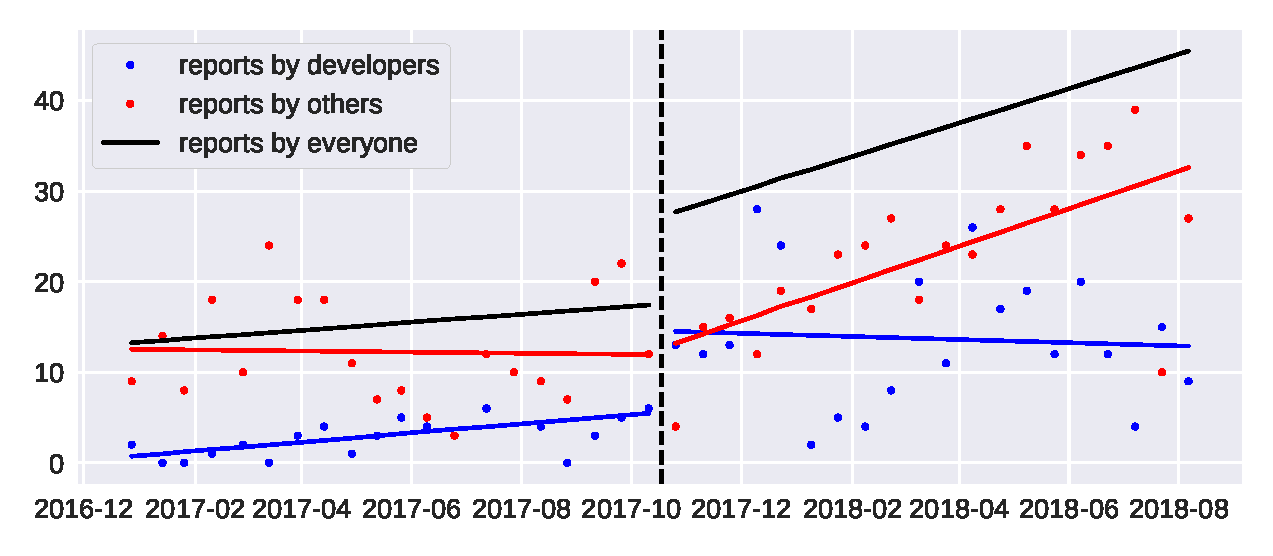
\includegraphics[width=\textwidth]{bug_nb_rd.eps}
\caption{Number of bug reports by 15-day period before and after the migration (with fitting lines from the regression results).} \label{bug_nb_rd}
\end{figure}


\subsection{Impact on the number of distinct bug reporters}

Table~\ref{tab:reporters} gives the estimated impact of the switch on the number of bug reporters (i.e. number of people that report a bug during a given period). As before, each column shows the estimates for a different sub-sample. Fig.~\ref{reporter_nb_rd}  shows the number of bug reporters before and after the switch and the fitting lines correspond to the regression results. These results demonstrate that the switch to GitHub positively affected not just the number of bug reports but also the number of non-developer bug reporters, suggesting an impact in both the intensive (number of bugs reported per person) and the extensive margin (number of reporters) of bug reporting.

\begin{table}
\centering
\caption{Estimated impact of the switch on the number of reporters by 15-day period. Coefficients are highlighted if they are statistically significant with $p<0.1$ (*), $p<0.05$ (**) or $p<0.01$ (***). Standard error is in parentheses.}\label{tab:reporters}
\begin{tabular}{|r|c|c|c|}
\hline
&  Total & Developers & Others \\
\hline
$\mbox{\emph{After switch}}_p$ & 4.15 & 1.24 & 2.91 \\
& (2.52) & (0.974) & (2.46) \\
\hline
$\mbox{\emph{Relative date}}_p * \mbox{\emph{After switch}}_p$ & 0.289 & -0.156* & 0.444** \\
& (0.218) & (0.0843) & (0.213) \\
\hline
$\mbox{\emph{Relative date}}_p$ & 0.111 & 0.159** & -0.0489 \\
& (0.154) & (0.0596) & (0.151) \\
\hline
Constant & 12*** & 3.97*** & 8.04*** \\
& (1.84) & (0.714) & (1.81) \\
\hline
Observation number & 40 & 40 & 40 \\
\hline
\end{tabular}
\end{table}

\begin{figure}
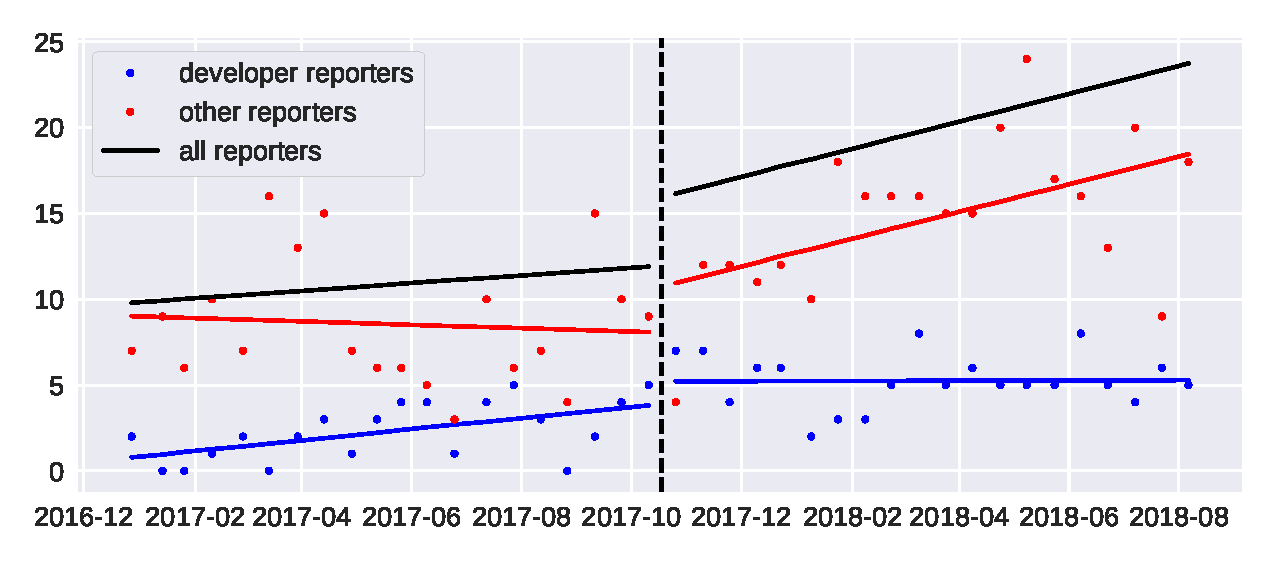
\includegraphics[width=\textwidth]{reporter_nb_rd.eps}
\caption{Number of distinct reporters by 15-day period before and after the migration (with fitting lines from the regression results).} \label{reporter_nb_rd}
\end{figure}

For non-developers, we see a statistically significant increase in the slope on the trend after the switch.
In particular, switching the bug reporting platform to GitHub increases the slope of the regression line by 0.44. This means that after the switch we will, in average, observe an increase of around one non-developer bug reporter each new month.
So for each period, there will be more non-developers who report a bug. This does not necessarily mean that these are people that never reported bugs before. It could also be that non-developer reporters start reporting more and more frequently. Again, this could be due to the increase of the bug reporting appeal, partly because of the platform, but also partly because they receive more feedback on their bug reports (as will suggest our results on comment numbers). 

For developers we see a slight but statistically significant (at 10\% level) negative effect on the slope of the trend after the switch. This means that, compared to the slope of the trend before the switch, the new trend has a lower slope. We wouldn't expect a significant change in the number of developers that report bugs because according to our definition there is a fixed number of developers, and they are already very active. Seeing the figure, we see  that the change in slope is due to a stabilization of a previous positive slope, probably meaning a reach of the maximum level of active developers per period. 

\subsection{Impact on the number of comments}

Table~\ref{tab:comment_nb} reports on the estimated impact of the bug tracker switch on the number of comments. We can see a statistically significant jump in the number of comments, which almost doubles. This is almost entirely due to comments by developers. This surge in bug comment activity shows that developers communicate more on the bug reports they receive, instead of just fixing and closing them. This means that the switch was beneficial in terms of transparency of the development, an evolution that is likely to give greater satisfaction to the bug reporters.

\begin{table}
\centering
\caption{Estimated impact of the switch on the number of comments. Coefficients are highlighted if they are statistically significant with $p<0.1$ (*), $p<0.05$ (**) or $p<0.01$ (***). Standard error is in parentheses.}\label{tab:comment_nb}
\begin{tabular}{|r|c|c|c|}
\hline
&  Total & Developers & Others \\
\hline
$\mbox{\emph{After switch}}_p$ & 84.7** & 72.2** & 12.5 \\
& (35.5) & (27.9) & (11.1) \\
\hline
$\mbox{\emph{Relative date}}_p * \mbox{\emph{After switch}}_p$ & -2.1 & -2.79 & 0.698 \\
& (3.07) & (2.41) & (0.957) \\
\hline
$\mbox{\emph{Relative date}}_p$ & 1.95 & 1.65 & 0.3 \\
& (2.17) & (1.71) & (0.677) \\
\hline
Constant & 86.6*** & 59.7*** & 26.9*** \\
& (26) & (20.4) & (8.11) \\
\hline
Observation number & 40 & 40 & 40 \\
\hline
\end{tabular}
\end{table}

\subsection{Impact on the number of distinct commentators}

Table~\ref{tab:commentators} and Fig.~\ref{commentator_nb_rd} show the estimated impact of the bug tracker switch on the number of distinct commentators by 15-day period. We can see a highly statistically significant jump in the number of non-developer commentators. This result is particularly interesting because it highlights a remarkable change in the way non-developers engage in the software developing process following the switch. What aspect of the GitHub platform creates this greater engagement remains to be studied but we hypothesize that this is due in large part to GitHub making it easier to subscribe to the bug report activity, and possibly also to the enhanced search.

\begin{table}
\centering
\caption{Estimated impact of the switch on the number of distinct commentators by 15-day period. Coefficients are highlighted if they are statistically significant with $p<0.1$ (*), $p<0.05$ (**) or $p<0.01$ (***). Standard error is in parentheses.}\label{tab:commentators}
\begin{tabular}{|r|c|c|c|}
\hline
&  Total & Developers & Others \\
\hline
$\mbox{\emph{After switch}}_p$ & 7.48*** & 0.763 & 6.72*** \\
& (2.63) & (0.684) & (2.3) \\
\hline
$\mbox{\emph{Relative date}}_p * \mbox{\emph{After switch}}_p$ & 0.238 & -0.0684 & 0.307 \\
& (0.228) & (0.0592) & (0.199) \\
\hline
$\mbox{\emph{Relative date}}_p$ & -0.00977 & 0.0368 & -0.0466 \\
& (0.161) & (0.0419) & (0.141) \\
\hline
Constant & 13.4*** & 7.04*** & 6.41*** \\
& (1.93) & (0.502) & (1.69) \\
\hline
Observation number & 40 & 40 & 40 \\
\hline
\end{tabular}
\end{table}


\begin{figure}
\includegraphics[width=\textwidth]{commentator_nb_rd.eps}
\caption{Number of distinct commentators by 15-day period before and after the migration (with fitted lines from the regression results).} \label{commentator_nb_rd}
\end{figure}

\section{Threats to validity}

\subsection{Internal threats}

The biggest concern that we have in our analysis is the fact that the date of the switch is close to the release of a new version of Coq. The release of version 8.7.0 took place on October 17\textsuperscript{th}, and the migration on October 18\textsuperscript{th}. Then, the hypothesis that there is no other discontinuity around the threshold of interest does not completely hold in our case. First, we can argue that not all our results are threatened: the jump in developer reports isn't because there is usually no peak in developer reports after new releases, same for the jump in non-developer commentators. Second, we can also argue that there should have been a similar (or higher) peak in the month before the switch since the first beta of 8.7 had been released then (and beta releases generally result in higher peaks). Third, we test for robustness by removing the two 15-day periods following the 8.7.0 release (and the switch) from our Regressions in Discontinuity. With these two periods removed, the regressions still give very close results with the same statistical significance.

We also conduct one standard robustness check for Regression in Discontinuity analysis by changing the time window of the analysis to fifteen and to ten periods before and after the switch. Our main results are robust to these changes.

\subsection{External threats}

This is only a case study on a very particular project (it is a software that can be used as a programming language, but requires expertise, that is developed mostly by French researchers, etc.). The only way to confirm the results we obtained would be to replicate this study on other examples of projects that went through a similar bug tracker switch.

\section{Conclusion and perspectives}

We have analyzed the impact of changing the bug reporting environment using a Regression in Discontinuity analysis with data from the switch of the Coq bug tracker from Bugzilla to GitHub.  We have shown that the switch increased the number of bug reports; started an increase of bug reporters per period (i.e. in a certain period there are more distinct reporters); increased the number of comments by developers and the number of distinct commentators per period among non-developers. These results fully validate our first and third hypotheses (increase of the number of bug reports, by developers in particular; improvement of the interaction between reporters and developers) and partially validate our second hypothesis (increase the diversity of bug reporters). We find particularly interesting the change in the number of comments by developers and in the number of distinct non-developer commentators because it shows a significant change in the dynamics of the bug reporting process that we believe can improve software development by engaging more people in the process, and by increasing openness and transparency.  

Given the lack of literature on the effects of bug tracking environments, interested researchers could expand our analysis in many different ways. Analyzing other outcomes (such as pull requests or the rapidity of bug resolution) could give interesting additional insights and help create a more complete picture of the mechanisms at play. It will be also interesting to analyze the effects on a longer period to see if the changes hold in the long run. Replicating our analysis for different contexts and software would increase the external validity of the results.

\scriptsize
\paragraph{}
\noindent \footnotesize{\textbf{Supporting data.}}
We provide our extraction and analysis code as a Jupyter notebook and the data we used as CSV files. We also provide the XML export of Bugzilla that was used for the migration and the migration script. Everything is available from \url{https://github.com/Zimmi48/impact-of-switching-bug-trackers}.
\paragraph{}
\noindent \footnotesize{\textbf{Authors' contributions.}}
TZ prepared and conducted the migration, designed and implemented the data extraction process, implemented the data analyses, and wrote part of the manuscript. AC designed the data analyses and wrote part of the manuscript.
\paragraph{}
\noindent\footnotesize{\textbf{Acknowledgements.}}
We would like to thank Ambre Williams for valuable advice and help on the design and implementation of the data analyses and C\'ecile Rottner for general advice, support, and proof-reading.

%
% ---- Bibliography ----
%
% BibTeX users should specify bibliography style 'splncs04'.
% References will then be sorted and formatted in the correct style.
%
\bibliographystyle{splncs04}
\bibliography{bib}
%
\end{document}
